
\documentclass[a4paper]{article}
\usepackage[left=1in, right=1in]{geometry}
\usepackage{graphicx}
\usepackage[colorlinks=true, urlcolor=blue, linkcolor=red]{hyperref}

\begin{document}

Saagnik Sarbadhikari, 50592327 

Marcus Hartman, 50398874

Bharath Reddy, 50563984

\begin{center}
  Project Phase 1
\end{center}

\begin{enumerate}
  \item Problem Statement (5pts, team)
  
  Title: Forecasting the Rental Housing Economy of Various Areas Using Machine Learning.

  Problem Statement: Develop a model that can accurately predict rent prices across various locations in the next few years. This will use past data along with future predictions on the economy, which can be used by various clients to find the most cost-effective location to rent.

  \bigbreak
  \underline{Potential of the Project}
  
  Explain the potential of your project to contribute to your problem domain. Discuss why this contribution is crucial?

  Our project aims to be useful in multiple aspects of the world. While our project isn't necessarily predicting the outcome of the economy in the next couple of years, we are aiming to get a gauge of the possibilities that the housing economy could take. This contribution aims to prove its usefulness to both current residents and people looking to move into a new area, as they will have a resource at their disposal that could aide in finding the best-fitting place to live a comfortable life economically.

  \item Ask Questions (10pts, individual)
  
  Saagnik:

\begin{enumerate}
    \item Could there be a larger increase in the gap of rent between a high-income state and one that is lower? Could we see people move to other states to save the money, but work remotely?

    \bigbreak
    This is a significant question as it poses a greater risk ever since the rise of remote work. We have seen people already do this, i.e., moving from New York City to Buffalo for this exact reason. I am wondering if this could be seen on a much larger scale, as rent continues to rise in those higher-income states.

    \item As rent continues to rise, could we see a decline of these prices to combat multi-family apartments?
    
    The significance of this question arises to illustrate the point of more people opting to live with multiple other people in order to save on rent in smaller buildings. Splitting rent for a three-bedroom apartment between seven people can be much more affordable than each having their own apartment—will the market react to this? What would this look like as prices keep rising? This is what an additional hypothesis can be formed to question. The best way to answer this question is to keep track of the price differences between one-bedrooms and multi-bedrooms in the future.
\end{enumerate}


  Marcus:

  \begin{enumerate}
    \item Could there be a larger increase in the gap of rent between a high-income state and one that is lower? Could we see people move to other states to save the money, but work remotely?
    
    \bigbreak
    This is a significant question as it poses a greater risk ever since the rise of remote work. We have seen people already do this, i.e. moving from New York City to Buffalo for this exact reason. I am wondering if this could be seen on a much larger scale, as rent continues to rise in those higher income states.

    \item As rent continues to rise, could we see a decline of these prices to combat multi-family apartments?
    
    The significance of this question arises to illustrate the point of more people opting to live with multiple other people in order to save on rent in smaller buildings. Splitting rent for a three-bedroom apartment between 7 people can be much more affordable than each having their own apartment-- will the market react to this? What would this look like as prices keep rising? This is what an additional hypothesis can be formed to question. The best way to answer this question is to keep track of the price differences between one-bedrooms and multi-bedrooms in the future.
  \end{enumerate}

  Bharath:

  \begin{enumerate}
    \item Given the higher mean and variation in rent prices in Los Angeles compared to Rochester, what implications does this have for the affordability of housing in these cities? 

    This question is significant as it highlights the economic disparity between high-cost living areas like Los Angeles and more affordable regions like Rochester. Understanding these implications can inform policymakers and potential renters about the sustainability of living in high-rent areas as economic conditions evolve.

    \bigbreak
    \item How does the consistency of rent prices in Rochester compared to the wider spread of rent prices in Los Angeles affect renters' choices in these cities?

    This question seeks to explore the impact of rent price stability on the decision-making process of potential renters. If Rochester offers more predictable rental costs, could it become a more attractive option for individuals seeking long-term housing stability, particularly as remote work becomes more common?

\end{enumerate}


  \item Data Retrieval (5pts, team)
  
  To help with individual questions that will be asked in Phase 2 and 3, our group has agreed to focus into two states per person. This will make it easier to strike our own findings, and can find different conclusions using the same model.

  \underline{Saagnik:}

  Rural:Seattle

  Urban:New York City


  \underline{Marcus:}

  Rural: Minnesota

  Urban: Texas

  \underline{Bharath:}

  Rural:Los Angeles

  Urban:Rochester

  \bigbreak
  \begin{center}
    Data Retrieval
  \end{center}

  Sources used (so far):
  \begin{enumerate}
    \item \href{https://www.huduser.gov/portal/datasets/fmr.html#null}{huduser.gov} - $40^{th}$ Percentile Rents (Historic)
    \item \href{https://www.zillow.com/research/data/}{zillow.com} - Current housing markets, estimations for an area
    \item \href{https://www.rentcast.io/api}{rentcast.io} - Additional market data for a zip code area
    \item \href{https://insideairbnb.com/get-the-data/}{insideairbnb.com} - AirBnB rentals by city
  \end{enumerate}

  Data retrieval consists of a couple calls to certain APIs. While the first two sources are free, rentcast unfortunately charges after the $31^{st}$ use of the month. Therefore, we only try to do this call once and store the result in the results/ folder we have for this. 

  The code can be found in the associated ipynb, where the following lines are found: 

  For huduser.gov:

  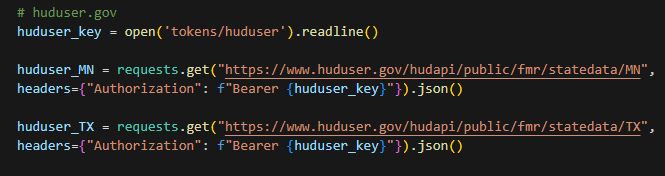
\includegraphics[scale=0.82]{huduser_retrieval.png}

  For zillow.com:

  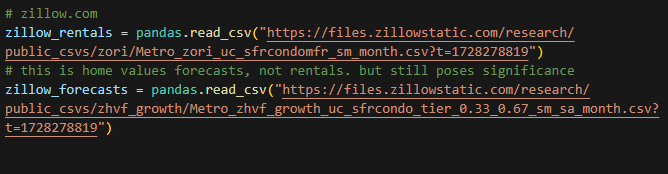
\includegraphics[scale=0.82]{zillow_retrieval.png}

  For rentcast.com:

  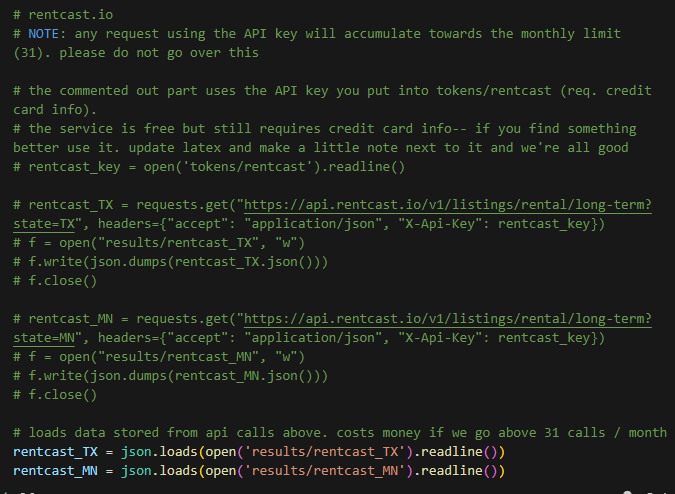
\includegraphics[scale=0.82]{rentcast_retrieval.png}

  For insideairbnb.com:

  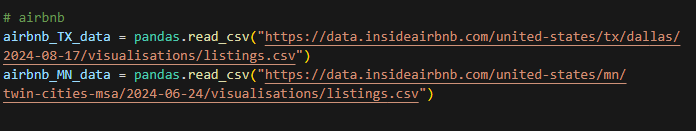
\includegraphics[scale=0.8]{airbnb_retrieval.png}

  \item Data Cleaning (10pts, team)
  
  For each dataset, we cleaned up all of the NaNs, converted every dataset into a similar JSON, and dropped any unnecessary columns pertaining to our problem. The reason why JSON is chosen is because pandas provides methods to convert such into pandas DataFrames, which provides exceptional methods that will aid in this project. Each are separated out by their source.

  For huduser.gov:

  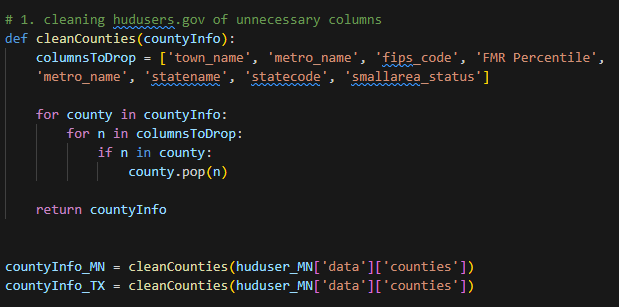
\includegraphics[scale=0.8]{huduser_cleaning.png}

  For zillow.com:

  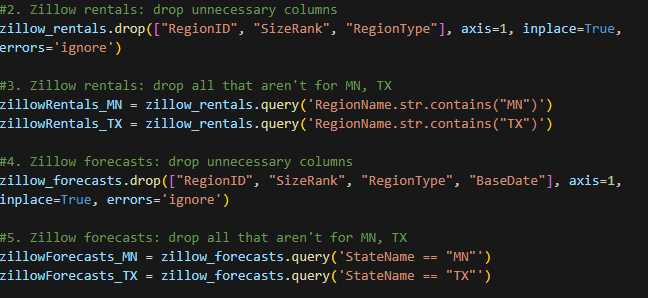
\includegraphics[scale=0.8]{zillow_cleaning.png}

  For rentcast.com:

  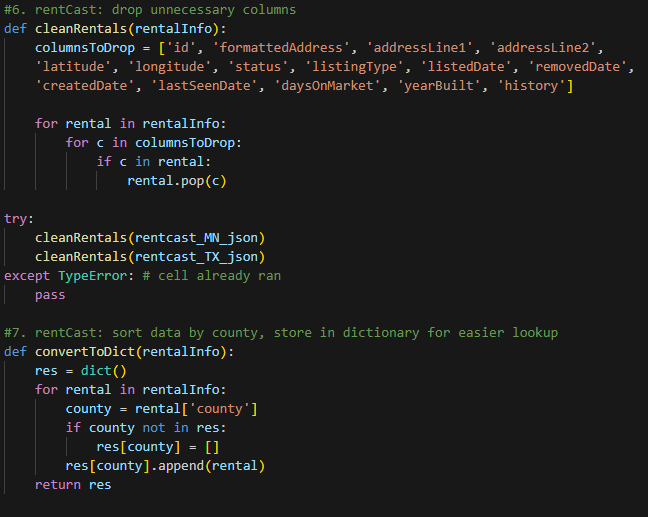
\includegraphics[scale=0.7]{rentcast_cleaning.png}

  For insideairbnb.com:

  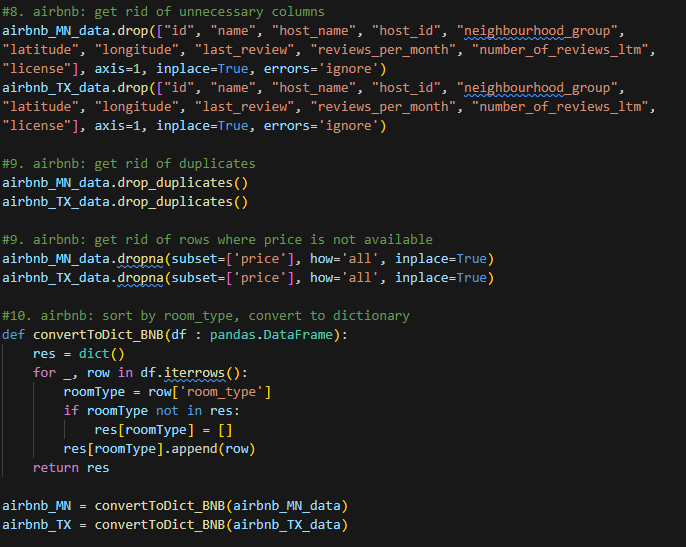
\includegraphics[scale=0.7]{airbnb_cleaning.png}


  \item Exploratory Data Analysis (20pts, individual)
  
  Saagnik:

\begin{enumerate}
    \item Out of the two states I have chosen, if I am looking at the data of New York compared to Seattle, I will see a higher mean and more variation of rent in New York because it is more economically active than Seattle.
    
    The following code is used to produce this example (data cleaning did most of the work here): 

    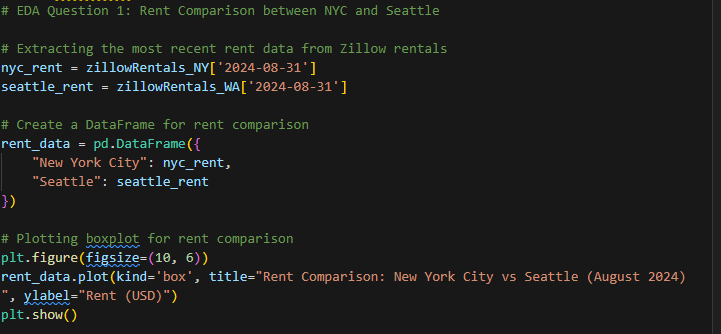
\includegraphics[scale=0.7]{Saagnik-Hypothesis-1-code.png}
    \bigbreak
    Which produces this graphic: 

    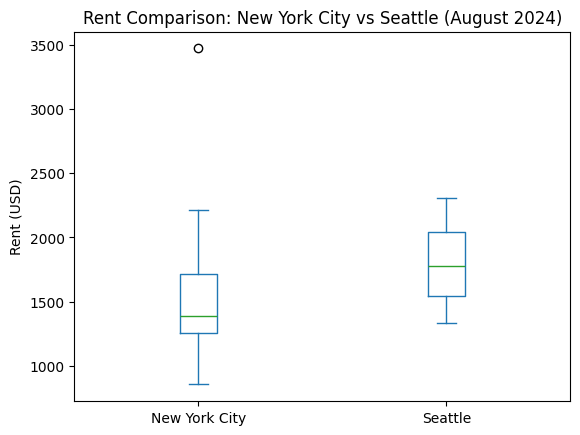
\includegraphics[scale=0.9]{Saagnik-Hypothesis-1.png}

    I tried to put an explanation in the code for this hypothesis. However, this will be expanded upon below. 
    
    The results show that New York experiences a higher mean rent and greater variation compared to Seattle, indicating a more dynamic rental market. This supports the hypothesis that economic activity influences rental prices and their distribution. Understanding these differences is crucial for predicting future rental trends and housing policy impacts.

    \item If New York's major boroughs have high rent, then there will be much lower rent outside of these boroughs because there is a lower standard of living comparatively. 
    
    Below is the code that will create the graphic: 

    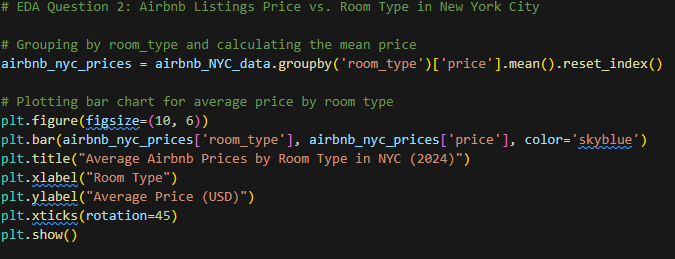
\includegraphics[scale=0.75]{Saagnik-Hypothesis-2-code.png}

    The graphic:

    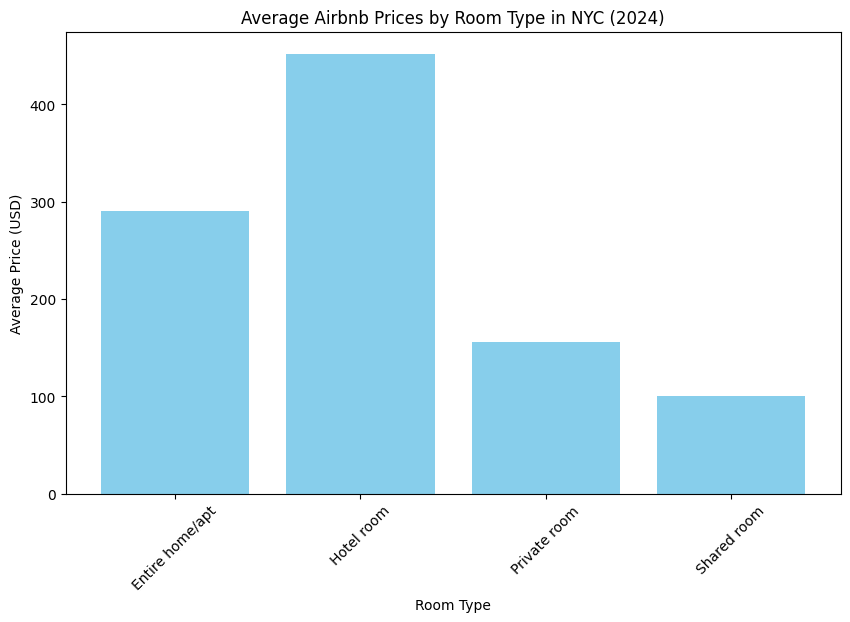
\includegraphics[scale=0.65]{Saagnik-Hypothesis-2.png}

    At first glance, this graphic may not seem to carry significant weight, but it reveals important insights about rent distribution and government assistance. The lines of efficiency indicate hard boundaries that illustrate the necessary rent efficiency compared to population. The upper limit approaches $3,000 per month, while the lower end hovers around $1,200. 

    Government assistance plays a pivotal role in maintaining rental efficiency, ensuring that landlords do not perceive their properties as financial losses. This assistance often translates to an additional $500 to $1,000, depending on various economic factors.

    The upper boundary signifies what tenants consider 'reasonable' rent within their economic means. Rental efficiency is a crucial metric that reflects this economic reality, and more detailed formulas can be found on the HUD user website. 

    In the context of predicting trends in future phases, this hypothesis reinforces the idea that economic conditions and governmental interventions significantly impact the rental landscape. Therefore, to achieve accurate predictive outcomes, it is vital to simulate an increasing gap in rental efficiency across different counties, accounting for economic growth disparities.
    
\end{enumerate}


  Marcus:

  \begin{enumerate}
    \item Out of the two states I have chosen, if I am looking at the data of Texas compared to Minnesota, I will see a higher mean and more variation of rent because Texas is more economically active than the other.
    
    The following code is used to produce this example (data cleaning did most of the work here): 

    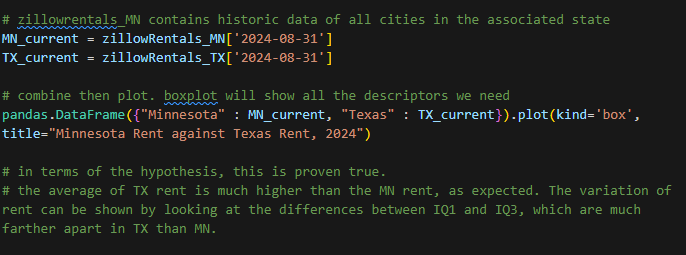
\includegraphics[scale=0.75]{Marcus-Hypothesis-1-code.png}
    \bigbreak
    Which produces this graphic: 

    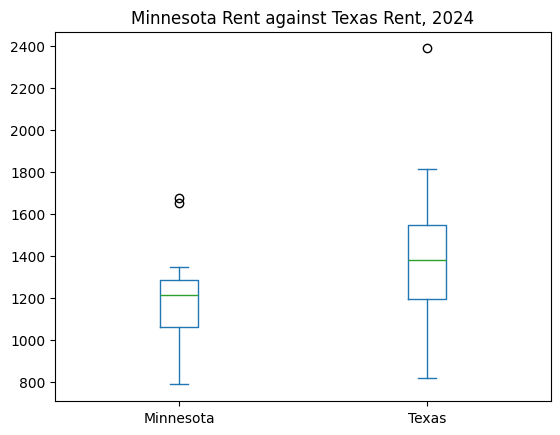
\includegraphics[scale=0.9]{Marcus-Hypothesis-1.png}

    I tried to put an explanation in the code for this hypothesis. However, this will be expanded upon below. 
    
    Minnesota experiences both a lower deviation and mean, signifying a much cheaper rent economy than Texas. This proves the hypothesis correct, and yields results that will be used in the later phases. The use of this stems from understanding the different economies in place, and how additional steps will need to be taken in order to predict economic growth in different areas. 


    \item If Minnesota's major cities have high rent, then there will be much lower rent outside of these cities because there is a lower standard of living comparatively. 
    
    Below is the code that will create the graphic: 

    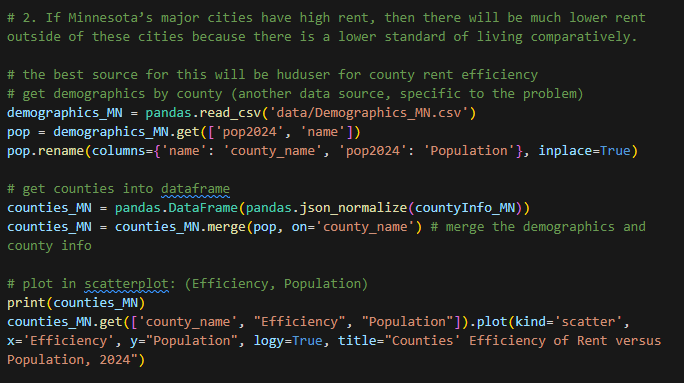
\includegraphics[scale=0.75]{Marcus-Hypothesis-2-code.png}

    The graphic:

    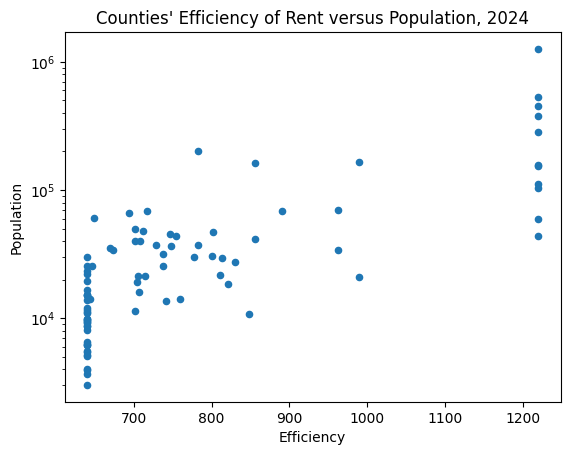
\includegraphics[scale=0.9]{Marcus-Hypothesis-2.png}

    Although at first this graphics doesn't seem to have any significance, a little bit of forward thinking into government assistance is necessary. The lines of efficiency represent hard boundaries that demonstrate the limits of necessary rent efficiency compared to population. On the higher end of this, we see this cap off at slightly above 1200 per month. On the lower end, this is closer to 600. 
    
    Government assistance is used to subsidize the rent efficiency in order for the owners to not consider the property a loss. This is what the line is, and often is around 300-550 additional provided (based on income and other factors).

    On the higher end, the barrier symbolizes what people will deem as 'reasonable' rent given the economic state that they can properly afford. Rental efficiency does take this into account, and the formula can be found on the huduser.gov website. 

    In terms of phase 2 and phase 3, this has a similar outcome compared to my first hypothesis. This shows the significance the economy and government assistance has on the rental climate. We cannot expect the lower efficient counties to not have increase government assistance while not experiencing some form of exponential economic growth in the higher efficient counties. In terms of predicting something of this nature, an increased gap will have to be simulated in order to garner accurate results of predictions. 
    
  \end{enumerate}

  Bharath:

  \begin{enumerate}
    \item Given the higher mean and variation in rent prices in Los Angeles compared to Rochester, what implications does this have for the affordability of housing in these cities? 

    This question is significant as it highlights the economic disparity between high-cost living areas like Los Angeles and more affordable regions like Rochester. Understanding these implications can inform policymakers and potential renters about the sustainability of living in high-rent areas as economic conditions evolve.

    \bigbreak
    \item How does the consistency of rent prices in Rochester compared to the wider spread of rent prices in Los Angeles affect renters' choices in these cities?

    This question seeks to explore the impact of rent price stability on the decision-making process of potential renters. If Rochester offers more predictable rental costs, could it become a more attractive option for individuals seeking long-term housing stability, particularly as remote work becomes more common?

\end{enumerate}

\end{enumerate}

\end{document}